\documentclass[a4paper,twoside,master.tex]{subfiles}
\begin{document}
\lecture{38}{Friday, November 15, 2019}{Infinite Chain of Coupled Harmonic Oscillators, Continued}

\subsubsection{The Classical Case, Continued}

Recall our Hamiltonian:
\begin{equation}
    H = \sum_j \left( \frac{ p^2_j}{2m} \frac{1}{2} m \omega^2 x_j^2 + \frac{1}{2 m \omega^2_j} (x_j - x_{j+1})^2 \right)
\end{equation}

When we looked at the Classical case, we introduced normal modes:
\begin{equation}
    x_j^{(k)}(t) = A e^{\imath (kj l - \omega t)}
\end{equation}

Now let's introduce ``normal coordinates'':
\begin{equation}
\xi(k, t) = \sum_j x_j(t) e^{- \imath kj l}
\end{equation}
We also need to introduce a similar transformation of momentum variables:
\begin{equation}
    \pi(k, t) = \sum_j p_j(t) e^{- \imath kj l}
\end{equation}

These are the Fourier transforms of the position and momentum coordinates, so we can alternatively write those as
\begin{equation}
    x_j(t) = \frac{l}{2 \pi} \int_{- \frac{\pi}{l}}^{ \frac{\pi}{l}} \xi(k, t) e^{\imath kj l}
\end{equation}
\begin{equation}
    p_j(t) = \frac{l}{2 \pi} \int_{- \frac{\pi}{l}}^{ \frac{\pi}{l}} \pi(k, t) e^{\imath kj l}
\end{equation}

\begin{theorem}{Parseval Theorem}
    The norm of a function equals the norm of its Fourier transform.
\end{theorem}
\begin{equation}
    \sum_{j=- \infty}^{\infty} x_j^2 = \frac{l}{2 \pi} \int_{- \frac{\pi}{l}}^{ \frac{\pi}{l}} \norm{\xi(k,t)}^2
\end{equation}
\begin{equation}
    \sum_{j=- \infty}^{\infty} p^2 = \frac{l}{2 \pi} \int_{- \frac{\pi}{l}}^{ \frac{\pi}{l}} \norm{\pi(k,t)}^2
\end{equation}
We can also find
\begin{align}
    \sum_j (x_j - x_{j+1})^2 &= \frac{l}{2 \pi} \int (1 - e^{\imath k l}) \norm{\xi(k,t)}^2 \dd{k} \\
    &= \frac{l}{2 \pi} \int \dd{k} 4 \sin[2](\frac{kl}{2}) \norm{ \xi(k,t)}^2
\end{align}

We can now rewrite the Hamiltonian as
\begin{equation}
    H = \frac{l}{2 \pi} \int \dd{k} \left\{ \frac{1}{2m} \norm{ \pi(k,t)}^2 + \frac{1}{2} m \Omega^2 \norm{ \xi(k,t)}^2  \right\}
\end{equation}
where $ \Omega^2 = \Omega^2(k) = \omega^2 + 4 \omega_1^2 \sin[2](\frac{kl}{2}) $.

Let's introduce a complex variable $ \alpha(k,t) = \frac{1}{\sqrt{2}} \left[ \sqrt{\frac{m \Omega}{\hbar}} \xi(k,t) + \imath \frac{1}{\sqrt{m \hbar \Omega}} \pi(k,t) \right] $ (reminiscent of the creation and annihilation operators in a quantum space):
\begin{equation}
    H = \frac{l}{2 \pi} \int \dd{k} \frac{1}{2} \hbar \Omega(k) [ \alpha(k,t) \alpha^*(k,t) + \alpha(-k,t) \alpha^*(-k,t)]
\end{equation}

\subsubsection{The Quantum Case}

We now have to worry about non-commutation of the position and momentum variables, which are now promoted to quantum operators.
\begin{equation}
    \comm{ \vu{X}_{j_1}}{ \vu{P}_{j_2}} = \imath \hbar \delta_{j_1,j_2}
\end{equation}
\begin{equation}
    \vu{\Xi}(k) = \sum_j \vu{X}_j e^{- \imath k_j l} = \vu{\Xi}^\dagger(-k)
\end{equation}
\begin{equation}
    \vu{\Pi}(k) = \sum_j \vu{P}_j e^{- \imath k_j l} = \vu{\Pi}^\dagger(-k)
\end{equation}
\begin{equation}
    \comm{ \vu{\Xi}(k)}{ \vu{\Pi}^\dagger(k')} = \imath \hbar \frac{2 \pi}{l} \delta(k - k')
\end{equation}
We can now define a ladder operator similar to $ \alpha $ in the classical case:
\begin{equation}
    \vu{a}(k) = \frac{1}{\sqrt{2}} \left[ \sqrt{\frac{m \Omega(k)}{\hbar}} \vu{\Xi}(k) + \imath \frac{1}{\sqrt{m \hbar \Omega}} \vu{\Pi}(k) \right]
\end{equation}
so the quantum Hamiltonian can be written
\begin{equation}
    \vu{H} = \frac{l}{2 \pi} \int \dd{k} \underbrace{\frac{1}{2} \hbar \Omega(k) \left\{ \vu{a}(k) \vu{a}^\dagger(k) + \vu{a}^\dagger(k) \vu{a}(k) \right\}}_{\vu{H}(k)}
\end{equation}
or
\begin{equation}
    \vu{H} = \frac{l}{2 \pi} \int \dd{k} \vu{H}(k)
\end{equation}
We see that this Hamiltonian in $ k $-space is equivalent to $ \vu{H}(k) = \hbar \Omega \left(\overbrace{ \vu{a}^\dagger(k) \vu{a}(k)}^{ \vu{N}(k)} + \frac{1}{2} \right) $.

We say that this number operator counts the number of phonons, where each phonon just refers to the number of times the system has been excited. One practical application of this is neutron scattering, where a neutron with some incident energy and momentum is scattered off of a crystal lattice. If we label the incident energy $ E_i $ and momentum $ \va{p}_i = \hbar \va{k}_i $ and the outgoing energy and momentum $ E_o $ and $ \va{p}_o = \hbar \va{k}_o $, we can create a plot, for different incoming momenta, $ \Delta E = E_o - E_i $ and $ \Delta \va{k} = \va{k}_o - \va{k}_i $ (see \Cref{fig:neutron_scattering})

\begin{figure}[h]
    \centering
    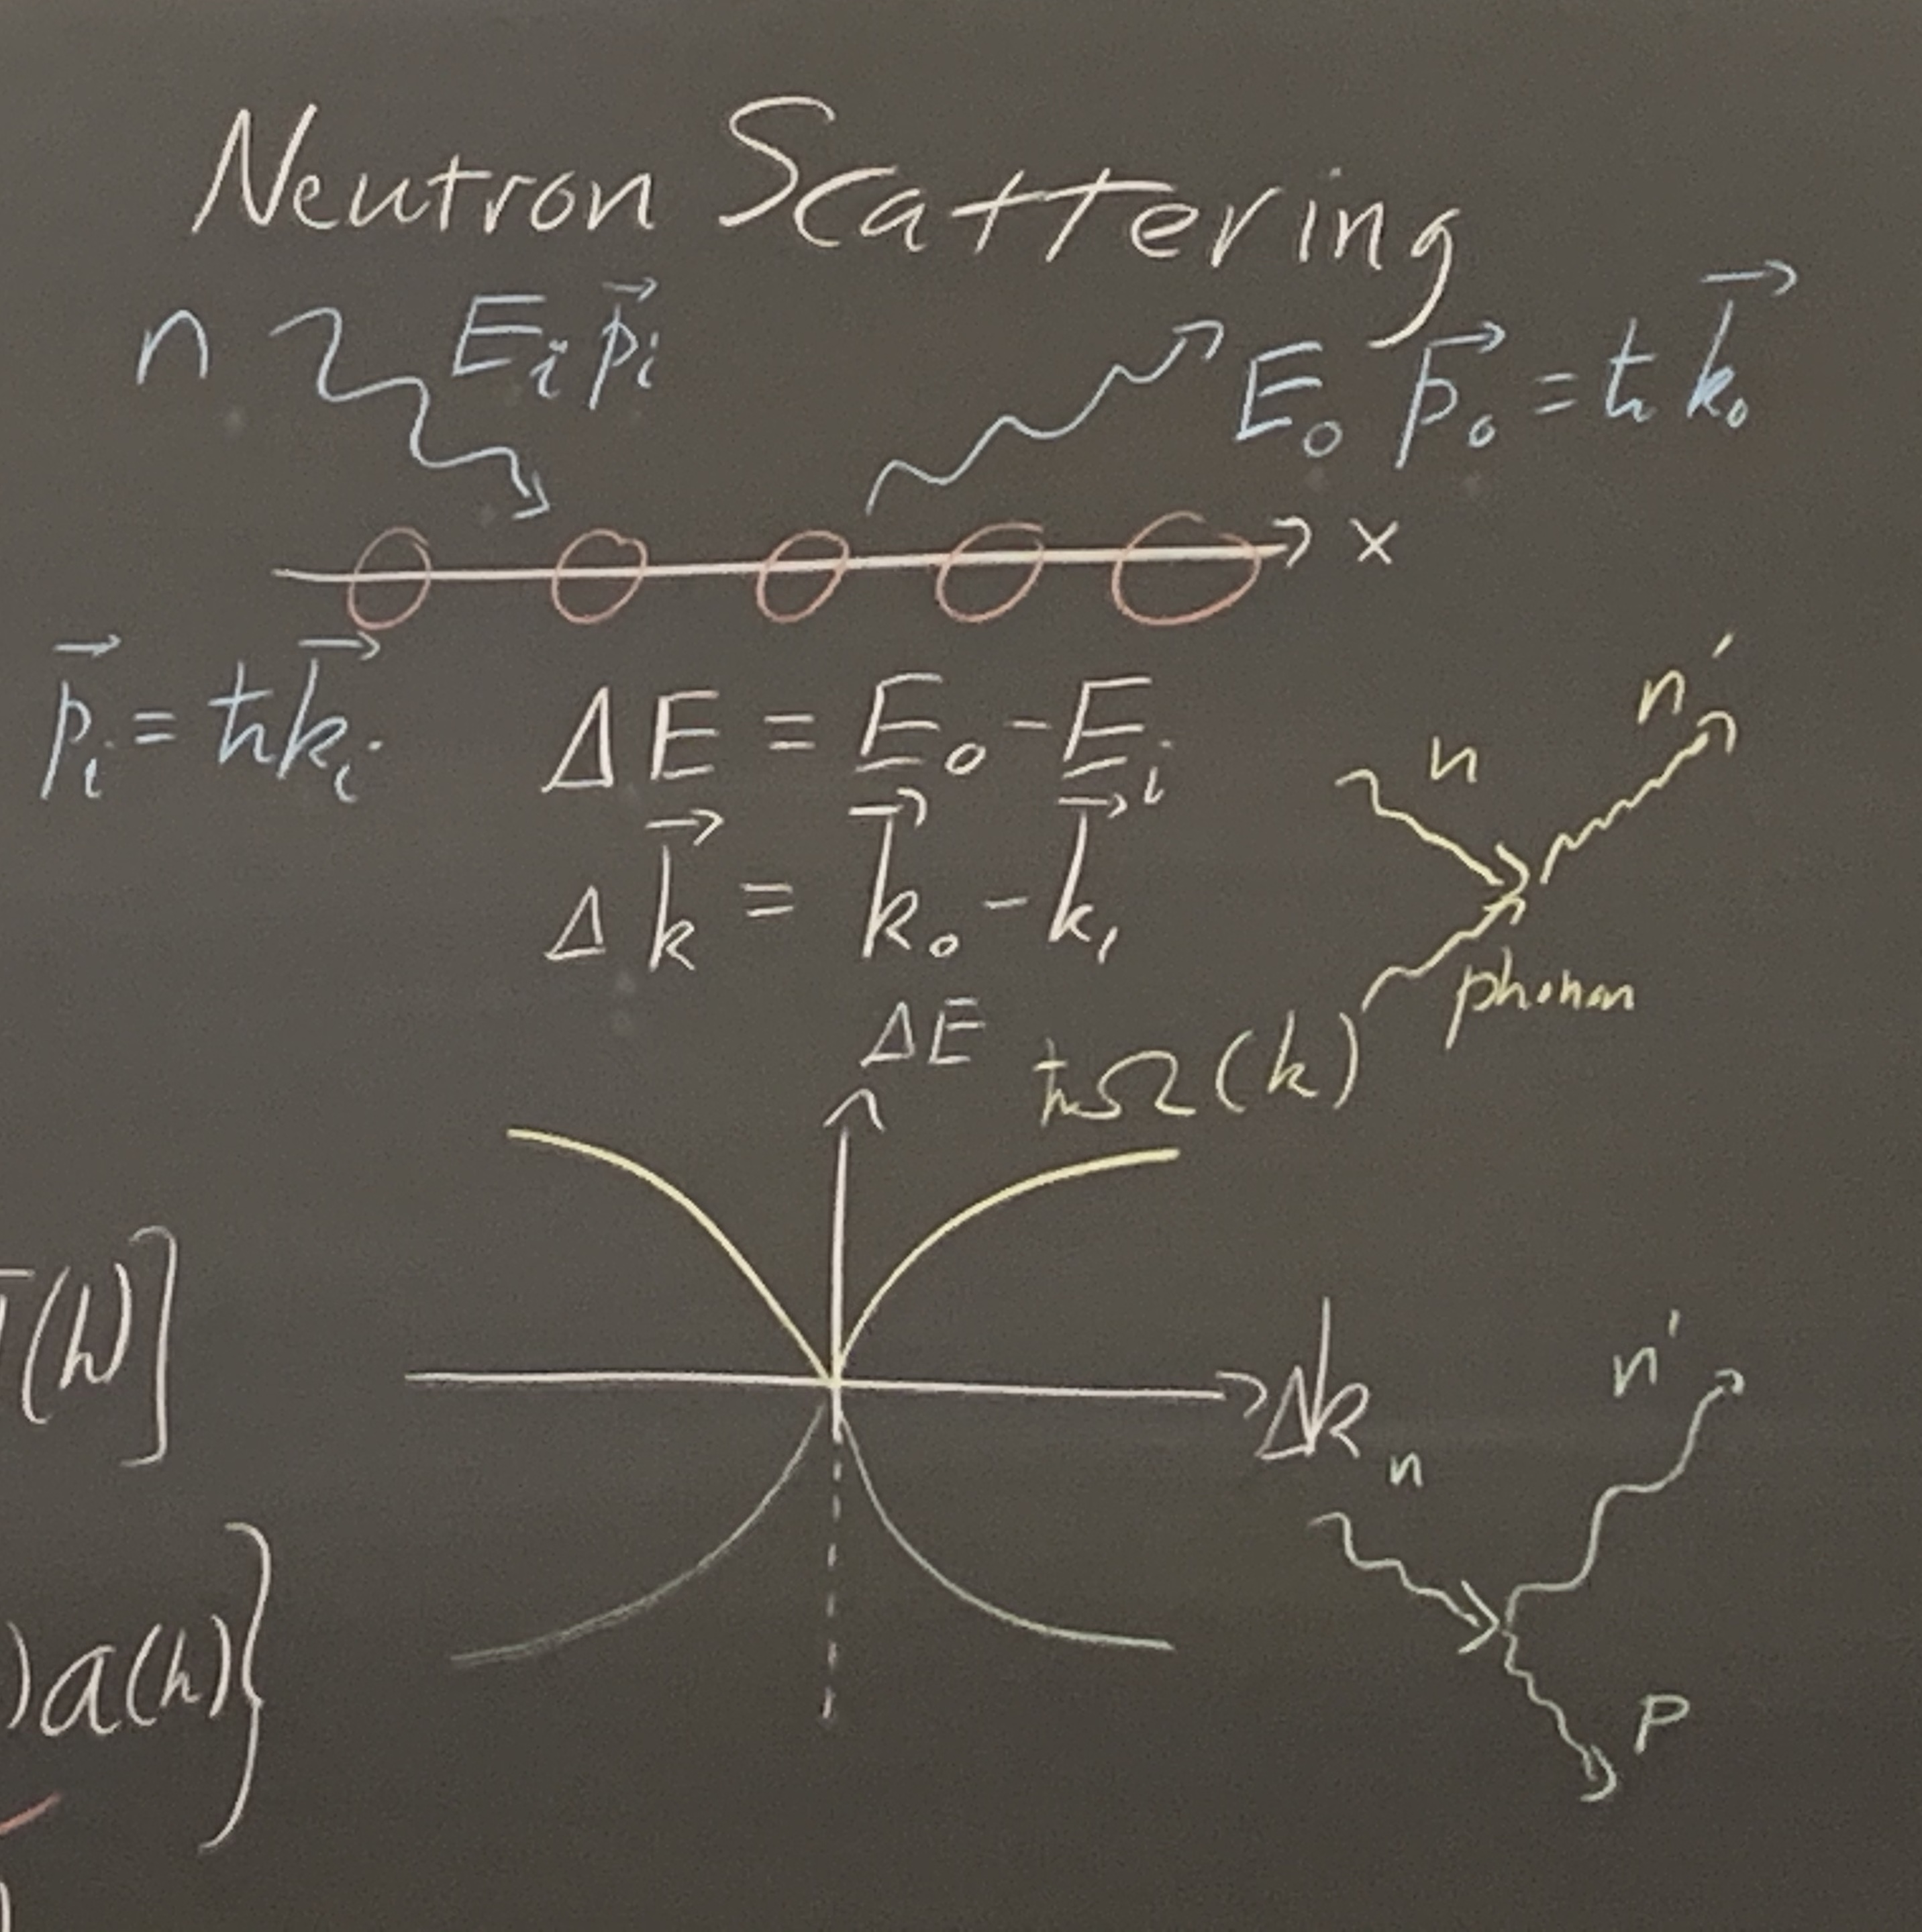
\includegraphics[width=\textwidth/2]{figures/lec_38_neutron_scattering.jpg}
    \caption{Plot of $ \hbar \Omega(k) $ illustrating the interaction of neutrons with a crystal lattice. Negative values correspond to the creation of a phonon while positive values mean a phonon has been absorbed by the scattered neutron, giving it more energy when it leaves the system.}
    \label{fig:neutron_scattering}
\end{figure}

\section{Thermal Equilibrium}
\label{sec:thermal_equilibrium}

Let's create a density operator $ \vu{\rho} = \frac{1}{\vu{Z}} e^{- \frac{\vu{H}}{kT}} $ where $ \vu{Z} = \Tr[e^{- \frac{\vu{H}}{kT}}] $. For a simple harmonic oscillator, we had $ E_n = \left( n + \frac{1}{2} \hbar \omega \right) $ for eigenstates $ \ket{n} $. Here,
\begin{align}
    \vu{Z} &= \sum_n \ev{e^{- \frac{\vu{H}}{kT}}}{n} \\
    &= e^{- \frac{\hbar \omega}{2kT}} \sum_{n=0}^{\infty} (e^{- \frac{\hbar \omega}{kT}})^{n} \\
    &= \frac{e^{- \frac{\hbar \omega}{2kT}}}{1 - e^{- \frac{\hbar \omega}{kT}}} \\
    &= \Tr[ \vu{\rho} \vu{H}] \\
    &= \frac{1}{ \vu{Z}} \sum_n \left( n + \frac{1}{2} \right) \hbar \omega e^{-E_n} \\
    &= \ev{ \vu{H}}
    &= \frac{\hbar \omega}{2} + \frac{1}{e^{\frac{\hbar \omega}{kT}} - 1}
\end{align}
The expectation value of the Hamiltonian here includes the zero-point energy.

We can also see that the expectation value of the number operator is
\begin{equation}
    \ev{ \vu{N}} = \frac{1}{e^{\frac{\hbar \omega}{kT}} - 1}
\end{equation}

Note that at low temperature, $ \ev{ \vu{N}} = 0 $ while at high temperature, $ \ev{ \vu{N}} \sim T $.

\end{document}
